\documentclass{beamer}
% \documentclass[handout]{beamer}
\usepackage{cuhkszbeamer}

% \CTEXoptions[today=old]

\title[Read Papers]{(Re-)Imag(in)ing Price Trends}
\subtitle{Forthcoming in \textit{Journal of Finance}}
\author[Zhiming]{
    Author:  Jingwen Jiang\footnote{Department of Computer Science, University of Chicago}\quad Bryan Kelly\footnote{Yale University, AQR Capital Management, and NBER}\quad Dacheng Xiu\footnote{Booth School of Business, University of Chicago}
    \vspace{0.1in}
    % \footnotesize{\href{mailto: zhimingmei@link.cuhk.edu.cn}{zhimingmei@link.cuhk.edu.cn}} \\
    % \footnotesize{School of Management and Economics}
    }
% \institute[CUHKSZ]{The Chinese University of Hong Kong, Shenzhen}
\date{\today}


\begin{document}


% Title page
\frame[plain]{\maketitle}

% Outline
\begin{frame}{Outline}
    \label{outline}
    \tableofcontents{}
\end{frame}

\section{Research Questions and Findings}
\begin{frame}
\frametitle{Research Questions}
\begin{itemize}
    \item What is the prediction method that can find the predictive patterns and further inform future theory?\\
    - Present the historical price as \textbf{an image} and model the predictive association between images and future returns using a \textbf{convolutional neural network (CNN).}
    \item Why is it beneficial to encode market data as an image rather than in the more standard time series numerical format?\\
    - \textbf{CNN} architectures are crafted for image analysis.\\
    - Allows the model to focus on \textbf{relational attributes} of the data. (Same intuition as humans, that we can more readily detect patterns in images)\\
    \item Why choose CNN?\\
    - CNN's ability to \textbf{extract predictive signals} from input data, makes it ideally suited to elicit patterns that underly financial markets.
\end{itemize}

\end{frame}

\begin{frame}{Findings}
\begin{itemize}
    \item Image-based CNN predictions are powerful and robust predictors of future returns. The predictive power is summarized in terms of out-of-sample portfolio performance.
    \item \textbf{Short-horizons: }Image-based return predictions, which constitute a technical price trend signal, are likely to be most potent over relatively short horizons. See Figure \ref{fig:1}
\end{itemize}
\begin{figure}[h]
    \centering
    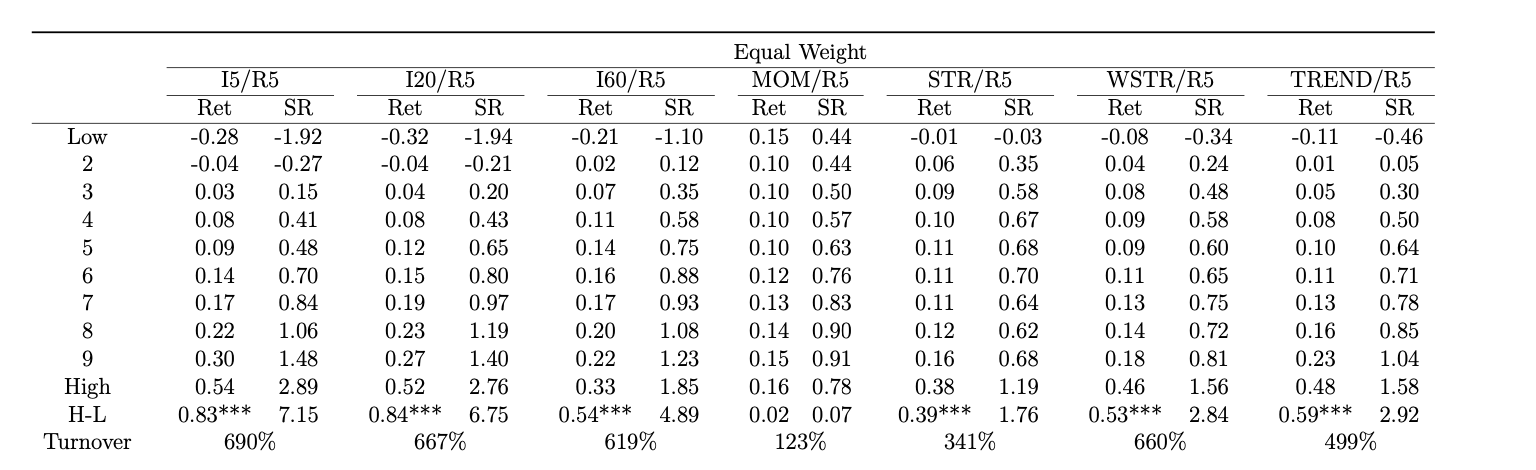
\includegraphics[width=.7\textwidth]{images/1 short-horizon portfolio performance.png}
    \caption{Short-horizon (One Week) Portfolio Performance}
    \label{fig:1}
\end{figure}
\begin{itemize}
    \item \textbf{Longer horizons: }The relative outperformance of CNN strategies is concentrated in the long leg of the H–L portfolio.
\end{itemize}
\end{frame}

\section{Methodology}
\subsection{Images}
\begin{frame}{Imaging Market Data}
\textbf{"OHLS" bars}:

The OHLS bars depict \textbf{daily opening, high, low, and closing prices}. And the image has a \textbf{20-day moving average closing price}. The bottom of the chart shows the daily \textbf{trading volume}. See Figure \ref{fig:2}

\begin{figure}[h]
    \centering
    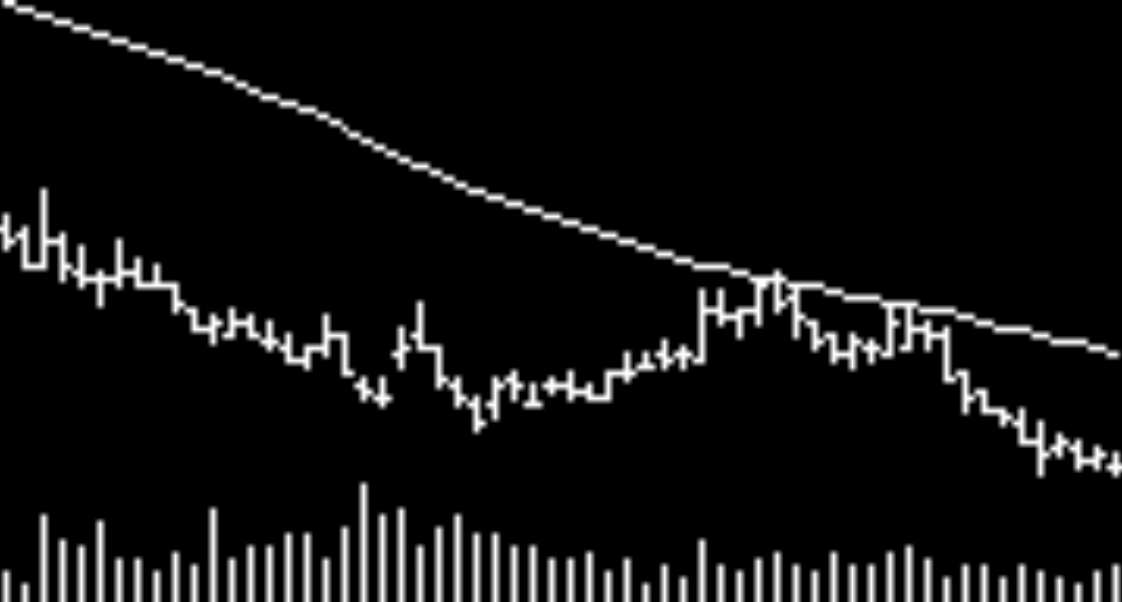
\includegraphics[width=.7\textwidth]{images/2 Generated OHLC Images with Volume Bar and Moving Average Line.png}
    \caption{Generated OHLC Images with Volume Bar and Moving Average Line
}
    \label{fig:2}
\end{figure}
\end{frame}

\begin{frame}{Why "OHLS" Bars?}
    \begin{itemize}
        \item The width of an \textit{n-day} image is thus \textit{3n} pixels.
        \item Impose a constant height for all images and scale the vertical axis so that the maximum and minimum of the OHLC path coincide with the top and bottom of the image. It conveys,\\
        - directional price trends\\
        - volatility information (high-low range over intervals other than a day are likewise beneficial for volatility inference.)
        \item Black-white image allows us to focus on two-dimensional pixel matrices
        \item This image (Figure \ref{fig:2}) concisely embeds a variety of information on \textbf{price trends, volatility, intraday and overnight return patterns, and trading volume.}
    \end{itemize}
\end{frame}

\subsection{CNN}
\begin{frame}{The Convolutional Neural Network Model}
    \begin{figure}[h]
        \centering
        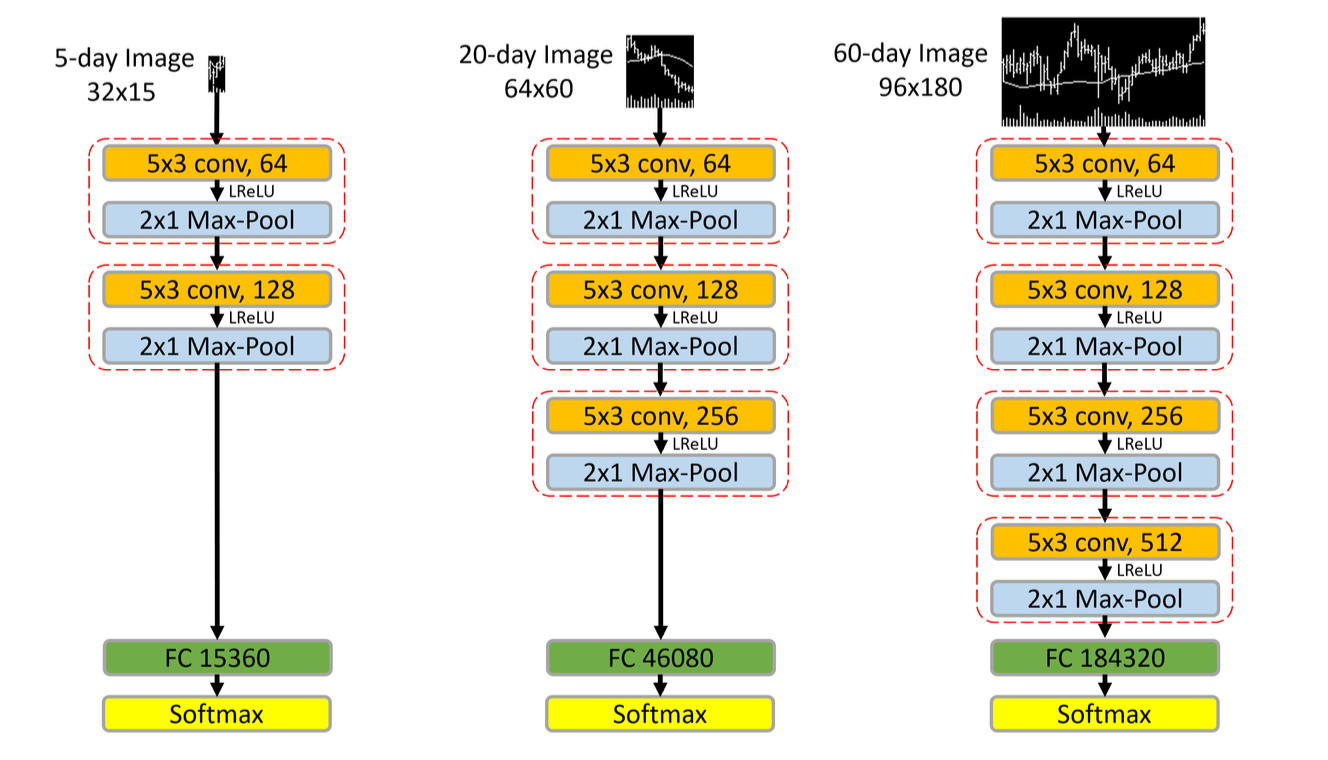
\includegraphics[width=\textwidth]{images/3 Diagram of CNN Models.png}
        \caption{Diagram of CNN Models}
        \label{fig:3}
    \end{figure}
\end{frame}

\begin{frame}{Image Representation}
\textbf{Note:} (Figure \ref{fig:4}, left) The table on top displays a \textbf{snippet of time series prices}. The bottom figure translates this time series into a black-and-white image where “255” represents a white pixel (corresponding to a price entry) and “0” represents empty space in the image.
    \begin{figure}[h]
        \centering
        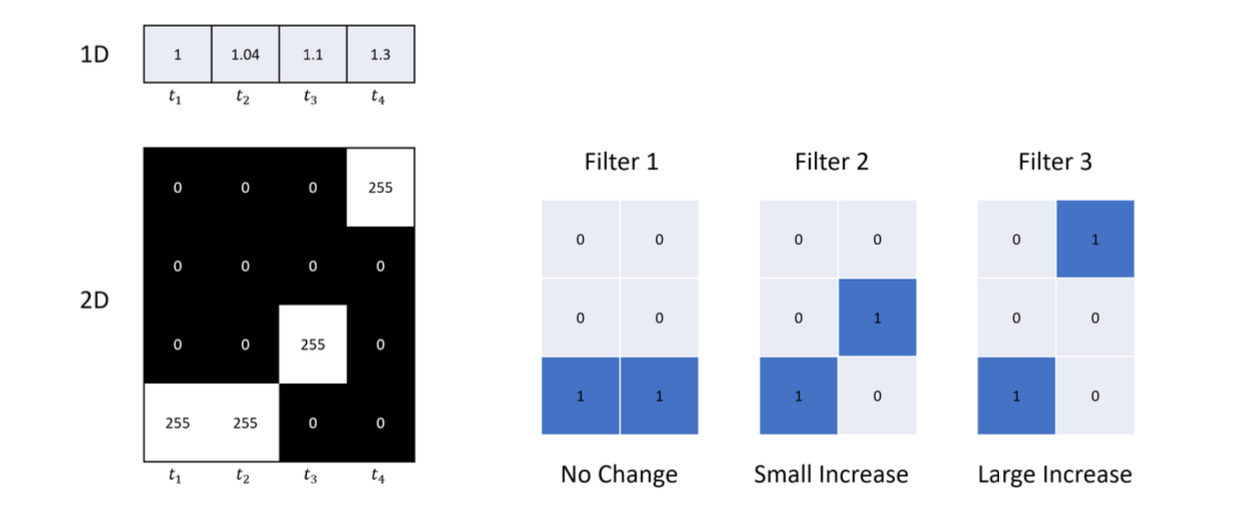
\includegraphics[width=.7\textwidth]{images/4 Convolutional Filters that Detect the Next Days Price Change.png}
        \caption{Convolutional Filters that Detect the Next Day’s Price Change}
        \label{fig:4}
    \end{figure}
The figure on the right demonstrates three 3 × 2 convolutional filters that detect no change, small increase, and large increase in price, respectively.
\end{frame}

\begin{frame}{Image vs. Time-Series Representation}
\textbf{Image Representation}
    \begin{itemize}
        \item Image representation makes it possible for a convolutional filter to capture non-linear spatial associations among various price curves. (Figure \ref{fig:4})
        \item “no change”, “small increase”, and “large increase” enter into an ultimate prediction with distinct weights.
    \end{itemize}
\textbf{Time-Series Representation}
\begin{itemize}
    \item Manually engineer features to jointly consider price direction and volatility.
    \item Require non-linear transformations of price series along the lines of stochastic volatility or GARCH models.
\end{itemize}
CNN \textbf{eliminates} these steps and extracts predictive patterns from data series within itself.
\end{frame}

\subsection{Model Training}
\begin{frame}{Model Training}
\begin{itemize}
    \item Randomly divide: 70\% images for training, and 30\% for validation
    \item Treat the prediction as the classification problem: the label for an image is defined as $y = 1$ if the subsequent return is positive, and $y = 0$ otherwise
    \item Training steps minimize the standard objective function for classification problems, \textbf{a cross-entropy loss function}.
\end{itemize}
  \begin{definition}[A Cross-Entropy Loss Function]
      It is defined as
      $$L(y, \hat{y}) = -y\log (\hat{y})-(1-y)\log(1-\hat{y})$$
      where $\hat{y}$ is the softmax output from the final step in the CNN.
  \end{definition}  
\end{frame}

\begin{frame}{Simulation Experiments}
    To investigate the performance of the finite sample, we use Monte Carlo simulations.

    \textbf{Objective}\footnote{See Internet Appendix IA.3 for more details (simulation process)}:
    \begin{itemize}
        \item Demonstrate how CNN models recognize patterns and make correct predictions in environments with various signal-to-noise ratios.
        \item Demonstrates how transfer learning helps improve longer-horizon predictions by exploiting the self-similarity in the sample path of prices.
    \end{itemize}
    \textbf{Conclusion:} CNN successfully detects complicated technical patterns in realistically low signal-to-noise data sets.
\end{frame}

\section{Model Interpretation}
\begin{frame}{Association with Other Predictors}
Figure \ref{fig:5} reports slope coefficients and $R^2$ from panel logistic regressions of CNN model forecasts on stock characteristics.
    \begin{figure}[h]
        \centering
        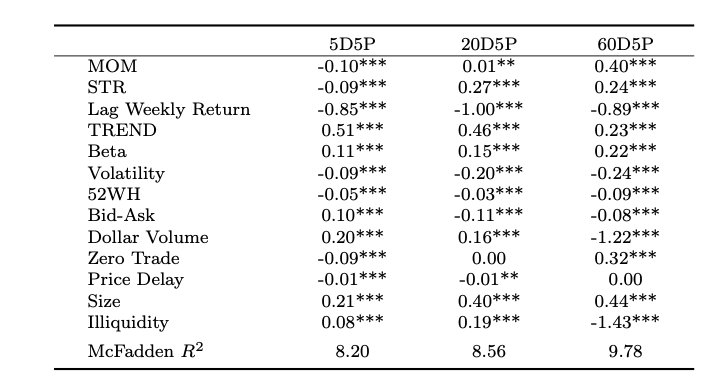
\includegraphics[width=.6\textwidth]{images/5 CNN Predictions and Standard Stock Characteristics.png}
        \caption{CNN Predictions and Standard Stock Characteristics}
        \label{fig:5}
    \end{figure}
Figure \ref{fig:5} shows that the CNN model has the ability to discern meaningful predictive information from images. CNN still manages to identify \textbf{trend-like features} and \textbf{liquidity features} in the raw images.
\end{frame}

\begin{frame}{Logistic Approximation}
\textbf{Question: }What do the CNN model detect in images to predict that are different from traditional stock-level predictors. 
    \begin{itemize}
        \item CNN is structured as a binary classifier, so the output is a probability. Logistic regression can be regarded as linear approximation of CNN.
        \item Scale the price series and volumes s.t. logistic regression is comparable with CNN.
    \end{itemize}
    For the regression:
    \begin{itemize}
        \item Dependent variable: the out-of-sample forecast generated by the CNN model for (5-day) images
        \item Independent variable: data underlying (5-day) images re-scaled to mimic the image representation
    \end{itemize}
The most important explanatory variables for the CNN forecast are the first lags of closing, high, and low prices.
\end{frame}

\section{Conclusions}
\begin{frame}{Conclusions}
    \begin{itemize}
        \item Image-based forecasts (based on CNN) in general outperform (and are in large part distinct from) traditional price trend signals in the asset pricing literature.
        \item Robustness: Transferability to international markets and other time scales.
        \item Our ideal research agenda is to develop a model that can translate visual data into an optimal portfolio in a way that mimics the \textbf{human perceptions and decision process.} $\to$ Understand market dynamics and form efficient portfolios.
    \end{itemize}
\end{frame}
\end{document}